\documentclass[11pt]{article}

\usepackage{amsmath}
\usepackage{amsfonts}
\usepackage{amssymb}

% Give ourself extra space for text
\usepackage[left = 2.2cm, right = 2.2cm, top = 1.8cm, bottom = 2.8cm]{geometry}

% Allows us to easily change the numbering system used in things like \begin{enumerate}. https://ctan.org/tex-archive/macros/latex/contrib/enumitem/
\usepackage[shortlabels]{enumitem}

% Turns table of contents, \refs, etc. into hyperlinks
\usepackage{hyperref}

% To include image, just use \includegraphics[scale=•]{relative path to image}
\usepackage{graphicx}
\graphicspath{ {./images/} }

% Common sets
\newcommand{\integers}{\mathbb{Z}}
\newcommand{\naturals}{\mathbb{N}}
\newcommand{\reals}{\mathbb{R}}

% Inverse hyperbolic functions
\DeclareMathOperator{\arcosh}{arcosh}
\DeclareMathOperator{\arsinh}{arsinh}
\DeclareMathOperator{\artanh}{artanh}

% I hat, J hat, K hat
\newcommand{\ihat}{\boldsymbol{\hat{\textbf{\i}}}}
\newcommand{\jhat}{\boldsymbol{\hat{\textbf{\j}}}}
\newcommand{\khat}{\boldsymbol{\hat{\textbf{k}}}}

% Better vectors (for single characters)
\renewcommand{\vec}[1]{\mathbf{#1}}

% Allows us to number equations in \begin{align} statements, etc.
\newcommand\numberthis{\addtocounter{equation}{1}\tag{\theequation}}

% NOTE: This means \section does NOT number sections, but ensures that they appear in the table of contents, which does not occur if simply \section* is used. From egreg @ https://tex.stackexchange.com/a/30225.
\setcounter{secnumdepth}{0} % sections are level 1

% This allows us to make augmented matrics using something like \begin{bmatrix}[cc|c]. Taken from Stefan Kottwitz at https://tex.stackexchange.com/questions/2233/whats-the-best-way-make-an-augmented-coefficient-matrix.
\makeatletter
\renewcommand*\env@matrix[1][*\c@MaxMatrixCols c]{%
  \hskip -\arraycolsep
  \let\@ifnextchar\new@ifnextchar
  \array{#1}}
\makeatother


\begin{document}
\title{ENG1005: Lecture 13}
\author{Lex Gallon}
\maketitle

\tableofcontents

\section*{Video link}
Click \href{https://echo360.org.au/lesson/G_8402119b-734b-4e1e-a3b4-7e907e86ddba_b944cecf-8ba5-40d3-a870-0243a0a9e78c_2020-04-21T15:58:00.000_2020-04-21T16:53:00.000/classroom#sortDirection=desc}{here} for a recording of the lecture.

\section{Linear systems of equations §5.5, 5.5.2}
\subsection*{Example}
\begin{enumerate}[ (a) ]
\item \textbf{1 equation and 2 unknowns.}
\[ -2x -3y = 4 \]
We solve this to get
\[ y = \frac{-1}{3}(4 + 2x),\ x \in \reals \]
which implies an infinite number of solutions. I.e.
\[ \{ (x, y) | x \in reals, y = \frac{-1}{3}(4 + 2x) \} \]

\item \textbf{2 equations and 2 unknowns.}
\begin{align*}
x + 2y &= 2 & (1) \\ 
2x + y &= 2 & (2) \\
\hline
x + 2y &= 2 & (1) \\ 
-3y &= -2 & (2) \rightarrow -2 \times (1) + (2) \\
\hline
x + 2y &= 2 & (1) \\ 
y &= \frac{2}{3} & (2) \rightarrow \frac{-1}{3}(2) \\
\hline
\end{align*}
Back-substitution to solve:
\[ x + \frac{4}{3} = 2 \Rightarrow x = \frac{2}{3} \text{ is the unique solution to the given equations} \]

\begin{center} 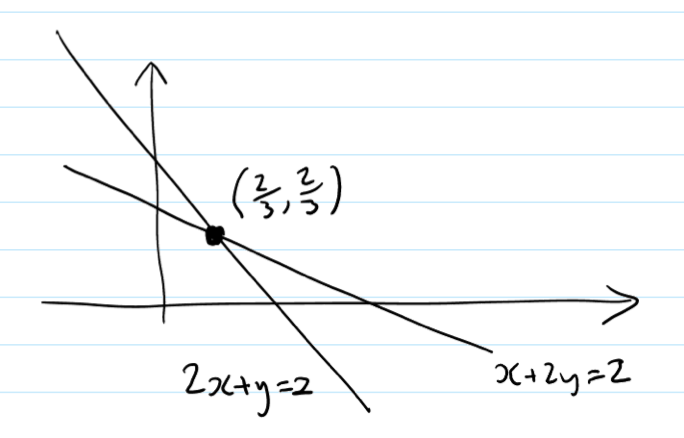
\includegraphics[scale=0.5]{linear_system_intersect} \end{center}

Since this system of equations has at least one solution, we call it a \textbf{consistent} system (same goes for that of part (a)).

(b.2)
\begin{align*}
\frac{1}{2}x + 2y &= 1 & (1) \\
-x - 4y &= 0 & (2) \\
\hline
\frac{1}{2}x + 2y &= 1 & (1) \\
0 &= 1 & (2) \rightarrow 2 \times (1) + (2)
\end{align*}
This contradiction implies no solution! This also means this is an \textbf{inconsistent} system.

\begin{center} 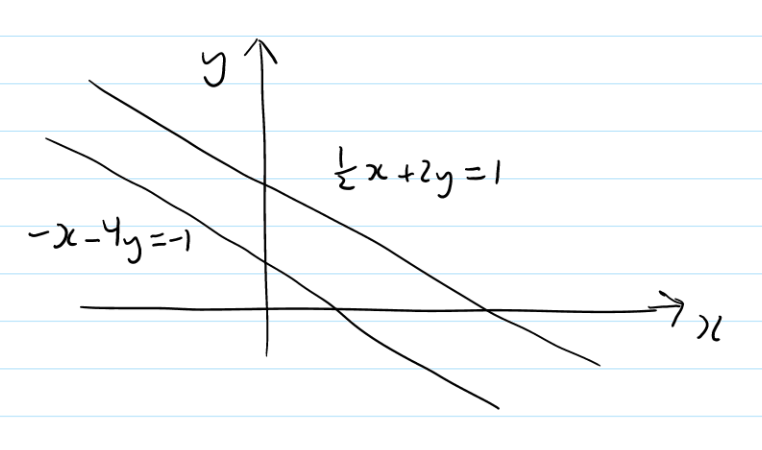
\includegraphics[scale=0.5]{linear_system_parallel} \end{center}


\end{enumerate}

\subsection{Definition}
A linear system of $m$-equations in $n$-unknowns is a set of equations of the form
\[ a_{11}x_1 + a_{12}x_2 + a_{13}x_3 + ... + a_{1n}x_n = b_1    \]
\[ a_{21}x_1 + a_{22}x_2 + a_{23}x_3 + ... + a_{2n}x_n = b_2 \]
\[ \vdots \]
\[ a_{m1}x_1 + a_{m2}x_2 + a_{m3}x_3 + ... + a_{mn}x_n = b_m \]
This system is called \textbf{consistent} if there exists at least 1 solution, and otherwise, it is called \textbf{inconsistent}.

\subsection*{Possible outcomes}
\begin{enumerate}[ (i) ]
\item No solution.
\item A unique solution.
\item An infinite number of solutions.
\end{enumerate}

\section{Elementary row operations §5.2.2}
Given a linear system of equations, we are free to:
\begin{enumerate}[ (1) ]
\item Multiply any one equation by a non-zero scalar $\lambda \in \reals$.
E.g.
\begin{align*}
3x + 2y - z &= 1 & (1) & & x + \frac{2}{3}y - \frac{1}{3}z &= \frac{1}{3} & (1) \rightarrow \frac{1}{3}(1) \\
4x - y + 2z &= -2 & (2) & \Leftrightarrow & 4x - y + 2z &= -2 & (2) \\
-x + y + z &= 4 & (3) & &  -x + y + z &= 4 & (3)
\end{align*}
\item Switch any two equations.
\begin{align*}
3x + 2y - z &= 1 & (1) & & -x + y + z &= 4 & (1) \rightarrow (3) \\
4x - y + 2z &= -2 & (2) & \Leftrightarrow & 4x - y + 2z &= -2 & (2) \\
-x + y + z &= 4 & (3) & &  3x + 2y - z &= 1 & (3) \rightarrow (1)
\end{align*}

\item Add $\lambda$ times one equation to another.
\begin{align*}
3x + 2y - z &= 1 & (1) & & 5y + 2z &= 13 & (1) \rightarrow 3 \times (3) + (1) \\
4x - y + 2z &= -2 & (2) & \Leftrightarrow & 4x - y + 2z &= -2 & (2) \\
-x + y + z &= 4 & (3) & &  -x + y + z &= 4 & (3)
\end{align*}

\end{enumerate}

\section{Matrices §5.2.1}
An $m \times n$ matrix is an $m$ by $n$ array of real numbers (complex numbers are allowed but whatever).

\[ A = [A_{ij}] \]
All $A_{ij}$ are the \textbf{coefficients} of the array $A$.

\[
[ A_{ij}] = 
\begin{bmatrix}
A_{11} & A_{12} & ... & A_{1n} \\
A_{21} & A_{22} & ... & A_{2n} \\
A_{31} & A_{32} & ... & A_{3n} \\
\vdots & \vdots & \ddots & \vdots \\
A_{m1} & A_{m2} & ... & A_{mn}
\end{bmatrix}
\]
where $1 \leq i \leq m$ is the row index and $1 \leq j \leq n$ is the column index.

\subsection{Definition}
Given a linear system of equations
\[ a_{11}x_1 + a_{12}x_2 + a_{13}x_3 + ... + a_{1n}x_n = b_1    \]
\[ a_{21}x_1 + a_{22}x_2 + a_{23}x_3 + ... + a_{2n}x_n = b_2 \]
\[ \vdots \]
\[ a_{m1}x_1 + a_{m2}x_2 + a_{m3}x_3 + ... + a_{mn}x_n = b_m \]

then the matrix
\[
[ A_{ij}] = 
\begin{bmatrix}[cccc|c]
a_{11} & a_{12} & ... & a_{1n} & b1 \\
a_{21} & a_{22} & ... & a_{2n} & b2 \\
\vdots & \vdots & \ddots & \vdots & \vdots \\
a_{m1} & a_{m2} & ... & a_{mn} & b_m
\end{bmatrix}
\]
is known as the \textbf{augmented matrix} of the linear system. (Note, the vertical line isn't require but does nicely distinguish it from a general matrix).

\section{Gaussian elimination §5.5.2}
\subsection*{Example}
\begin{enumerate}[ (i) ]
\item
\begin{align*}
2x - y + z &= 1 \\
x + 2y - z &= -1 \\
-x - y - z &= 2
\end{align*}

Switch R1 with R2
\begin{align*}
x + 2y - z &= -1 \\
2x - y + z &= 1 \\
-x - y - z &= 2
\end{align*}

R3 becomes R1 + R3
\begin{align*}
x + 2y - z &= -1 \\
2x - y + z &= 1 \\
y -2z &= 1
\end{align*}

R2 becomes R2 - 2R1
\begin{align*}
x + 2y - z &= -1 \\
- 5y + 3z &= 3 \\
y -2z &= 1
\end{align*}

Switch R2 with R3
\begin{align*}
x + 2y - z &= -1 \\
y -2z &= 1 \\
- 5y + 3z &= 3
\end{align*}

R3 becomes 5R2 + R3
\begin{align*}
x + 2y - z &= -1 \\
y -2z &= 1 \\
-7z &= 8
\end{align*}

Now, with augmented matrices
\[
\begin{bmatrix}[ccc|c]
2 & -1 & 1 & 1 \\
1 & 2 & -1 & -1 \\
-1 & -1 & -1 & 2
\end{bmatrix}
\]
\[ R_1 \leftrightarrow R_2 \]
\[
\begin{bmatrix}[ccc|c]
1 & 2 & -1 & -1 \\
2 & -1 & 1 & 1 \\
-1 & -1 & -1 & 2
\end{bmatrix}
\]
\[R_3 \rightarrow R_1 + R_3 \]
\[
\begin{bmatrix}[ccc|c]
1 & 2 & -1 & -1 \\
2 & -1 & 1 & 1 \\
0 & 1 & -2 & 1
\end{bmatrix}
\]
\[ R_2 \rightarrow R_2 - 2R_1 \]
\[
\begin{bmatrix}[ccc|c]
1 & 2 & -1 & -1 \\
0 & -5 & 3 & 3 \\
0 & 1 & -2 & 1
\end{bmatrix}
\]
\[ R_2 \leftrightarrow R_3 \]
\[
\begin{bmatrix}[ccc|c]
1 & 2 & -1 & -1 \\
0 & 1 & -2 & 1 \\
0 & -5 & 3 & 3
\end{bmatrix}
\]
\[ R_3 \rightarrow 5R_2 + R_3 \]
\[
\begin{bmatrix}[ccc|c]
1 & 2 & -1 & -1 \\
0 & 1 & -2 & 1 \\
0 & 0 & -7 & 8
\end{bmatrix}
\]

\end{enumerate}

\title{ENG1005: Lecture 14}
\author{Lex Gallon}
\maketitle

\tableofcontents

\end{document}